\chapter{State of the art}
This chapter will go through relevant articles and already known knowledge on the subject.

\section{Current system}
%Describe current system more in depth.
The EMC2DB uses two operating systems, a RTOS for safety-critical applications and a GPOS for non-critical applications. A Virtual Machine Monitor (VMM) is used to alternate between safety-critical RTOS and non-critical GPOS. The RTOS is TOPPERS FMP kernel \cite{website:FMP}, and the GPOS is a custom modified Linux distribution. The VMM used is SafeG \cite{website:safeg}. It switches processor state via a hardware switch. A Field Programmable Gate Array (FPGA) as interface between processor and board. %TODO: Expand!

An overview of the system can be seen in Figure~\ref{fig:introduction_overview}.

\begin{figure}[H]
\centering
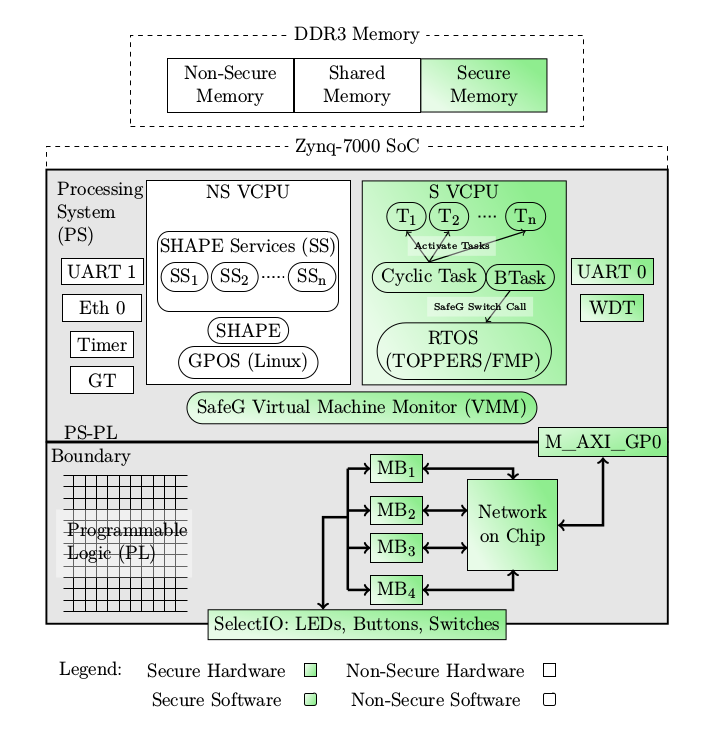
\includegraphics[width=\textwidth]{./img/introduction_overview.png}
\caption{System overview of the MCS in place.\cite{zaki2016}}\label{fig:introduction_overview}
\end{figure}

\section{Mixed criticality systems}
SotA regarding MCS.
